\chapter{RISC-V Architecture Overview}
\label{cha:riscv}

\lipsum[1]

\section{RISC-V Instruction Set Architecture}
\label{cha:riscv_isa}

\lipsum[1]

\begin{figure}[htbp]
  \centering
  \def\stackalignment{r}\stackunder{ 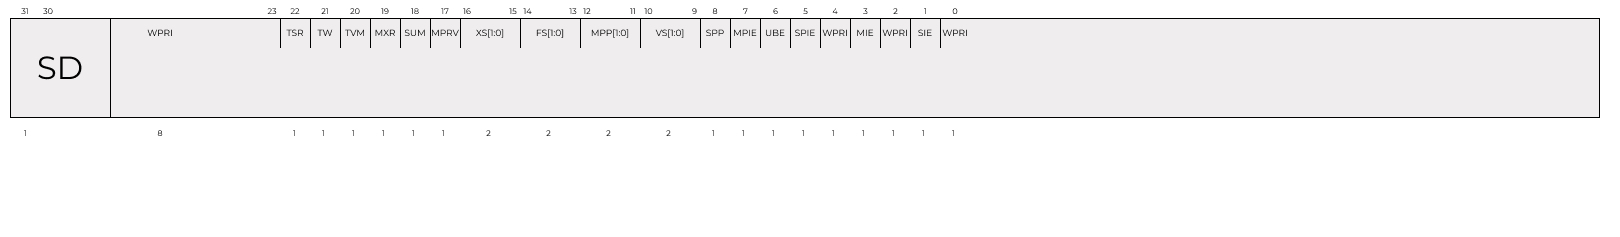
\includegraphics[width=.9\linewidth]{images/CSR-MSTATUS.png} } %
  {\scriptsize }
  \caption{University of Trento logo}
  \label{fig:csr}
\end{figure}

\section{Base Instruction Formats}
\label{cha:riscv_bif}

\lipsum[1]

\section{RISC-V Extensions}
\label{cha:riscv_extensions}

\lipsum[1]

\section{Exceptions, Traps and Interrupts}
\label{cha:riscv_eti}

\lipsum[1]

\section{RVWMO Memory Consistency Model}
\label{cha:riscv_rvwmo}

\lipsum[1]

\section{Privilege Levels}
\label{cha:riscv_privileges}

\lipsum[1]

\section{Control and Status Registers (CSRs)}
\label{cha:riscv_csr}

\lipsum[1]

\section{Physical Memory Protection (PMP)}
\label{cha:riscv_pmp}

\lipsum[1]

\section{RISC-V Toolchain}
\label{cha:riscv_toolchain}

\lipsum[1]